% This file was created by matlab2tikz.
%
\definecolor{mycolor1}{rgb}{0.89412,0.10196,0.10980}%
\definecolor{mycolor2}{rgb}{0.21569,0.49412,0.72157}%
%
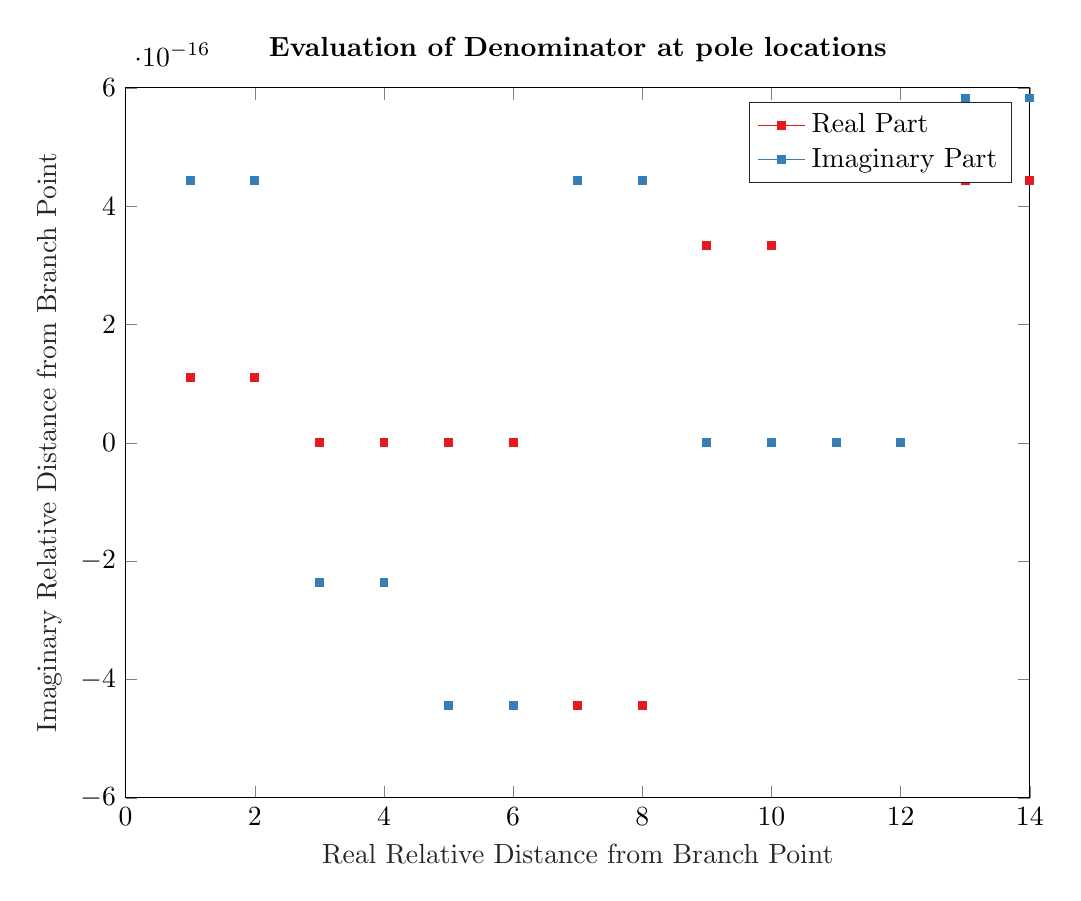
\begin{tikzpicture}

\begin{axis}[%
width=4.521in,
height=3.55in,
at={(0.758in,0.497in)},
scale only axis,
xmin=0,
xmax=14,
xlabel style={font=\color{white!15!black}},
xlabel={$\textrm{Real Relative Distance from Branch Point}$},
ymin=-6e-16,
ymax=6e-16,
ylabel style={font=\color{white!15!black}},
ylabel={$\textrm{Imaginary Relative Distance from Branch Point}$},
axis background/.style={fill=white},
title style={font=\bfseries},
title={Evaluation of Denominator at pole locations},
legend style={legend cell align=left, align=left, draw=white!15!black}
]
\addplot [color=mycolor1, draw=none, mark size=1.4pt, mark=square*, mark options={solid, fill=mycolor1, mycolor1}]
  table[row sep=crcr]{%
1	1.11022302462516e-16\\
2	1.11022302462516e-16\\
3	0\\
4	0\\
5	0\\
6	0\\
7	-4.44089209850063e-16\\
8	-4.44089209850063e-16\\
9	3.33066907387547e-16\\
10	3.33066907387547e-16\\
11	0\\
12	0\\
13	4.44089209850063e-16\\
14	4.44089209850063e-16\\
};
\addlegendentry{Real Part}

\addplot [color=mycolor2, draw=none, mark size=1.4pt, mark=square*, mark options={solid, fill=mycolor2, mycolor2}]
  table[row sep=crcr]{%
1	4.44089209850063e-16\\
2	4.44089209850063e-16\\
3	-2.35922392732846e-16\\
4	-2.35922392732846e-16\\
5	-4.44089209850063e-16\\
6	-4.44089209850063e-16\\
7	4.44089209850063e-16\\
8	4.44089209850063e-16\\
9	0\\
10	0\\
11	0\\
12	0\\
13	5.82867087928207e-16\\
14	5.82867087928207e-16\\
};
\addlegendentry{Imaginary Part}

\end{axis}
\end{tikzpicture}%